%arara: lualatex: { branch: developer, interaction: errorstopmode,
%arara: --> shell: yes, synctex: yes }
%arara: makeglossaries
%arara: biber: { options: [ '--wraplines' ] }

% \DocumentMetadata{testphase=phase-III}
\DocumentMetadata{lang=es-MX}

% NOTA: [<+->] se usa comio overlay para hacer que los bullets aparezcan uno por uno.


\documentclass[%
spanish,
progressbar=head,
% background=dark,
subsectionpage,
aspectratio=169
]{beamer}

\usepackage{babel}
\usepackage{microtype} 
\usepackage{tabularray}
\UseTblrLibrary{booktabs}
\usepackage{siunitx}
\usepackage{chemmacros}
\usepackage{multimedia}

\usepackage{glossaries}
\makeglossaries


\usepackage[style=authoryear,backend=biber,url=false]{biblatex}
    \addbibresource[location=remote]{http://127.0.0.1:23119/better-bibtex/export/collection?/1/I6GHQDZ5.biblatex}


\usepackage[skins]{tcolorbox}
    \tcbset{skin=beamer}

\usepackage{pgfpages}
\setbeamertemplate{note page}[plain]
% \setbeameroption{show only notes}
% \setbeameroption{show notes on second screen=right}

\usetheme{metropolis}

\metroset{%
subsectionpage=progressbar,
% background=dark
}

\newacronym{BPR}{BPR}{relación bolas-polvo}
\newacronym{AM}{AM}{aleación mecánica}
\newacronym{YSZ}{YSZ}{zirconia estabilida con itrio}
\newacronym{PCA}{PCA}{agentes de control del proceso}

% \usecolortheme{orchid}
% \title{Técnicas de preparación de materiales}
\title{Aleaciones mecánicas}
\subtitle{Variables del proceso de molienda}
\date{\today}
\author{Pablo E. Alanis}
\institute{Universidad Autónoma de Nuevo León, División de Posgrado\\Técnicas de preparación de materiales}
\begin{document}
\maketitle

\begin{frame}[allowframebreaks]{Outline}
    \tableofcontents
\end{frame}

\section{Variables del proceso de molienda}

\begin{frame}{Aleaciones mecánicas}
    
    \begin{columns}
    \column[c]{0.3\linewidth}
    \begin{itemize}
        \item<1-> El proceso de \emph{\gls{AM}} es complejo;
        \item<2-> para obtener el producto deseado, se tienen que \textit{optimizar} las condiciones de reacción.
    \end{itemize}
    \column[c]{0.7\linewidth}
    \begin{figure}
        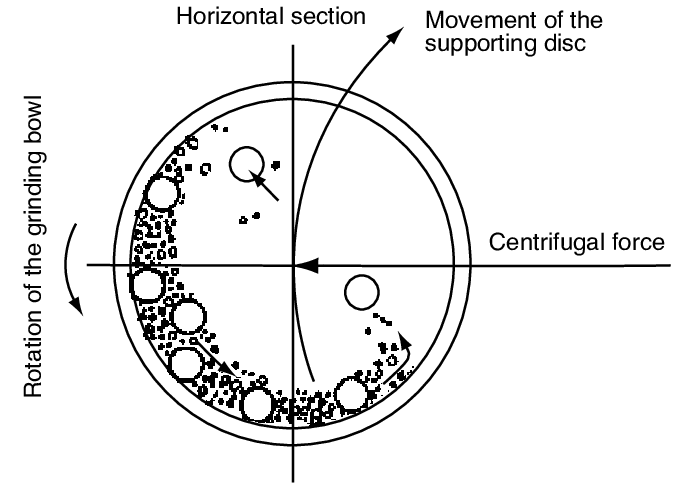
\includegraphics[width=0.8\linewidth]{figuras/milling.png}
        \caption{Esquema del proceso de molienda en un molino de bolas.}
    \end{figure}
\end{columns}
\end{frame}

\begin{frame}{Variables del proceso}
    Entre algunas de las variables que afectan la fase del producto final obtenido, se encuentran:

    \begin{itemize}[<+-| alert@+>]
        \item \emph{tipo} de molino;
        \item \emph{contenedor} del molino;
        \item \emph{velocidad} de molienda;
        \item \emph{tiempo} de molienda;
        \item \emph{tipo, tamaño y distribución} del medio de molienda;
        \item \emph{relación} en masa de bolas-polvo;
        \item \emph{que tan lleno} está el vial;
        \item \emph{atmósfera} de molienda;
        \item \emph{agente de control} del proceso;
        \item \emph{temperatura} de molienda.
    \end{itemize}
\end{frame}

\begin{frame}{Las variables no son aisladas}
\begin{itemize}[<+-| alert@+>]
    \item Estas variables no son necesariamente independientes;\\
    \item[] \textbf{por ejemplo:} el tiempo de molienda óptimo puede depender de: 
    \begin{enumerate}
        \item tipo de molino;
        \item tamaño del medio de molienda;
        \item temperatura de molienda;
        \item relación bolas-polvo, etc.
    \end{enumerate}
\end{itemize}
\end{frame}

\subsection{Tipos de molinos}

\begin{frame}{Selección de un molino}
    \begin{itemize}[<+-| alert@+>]
        \item Existen varios tipos de molinos que pueden usarse según el propósito;
        \item Estos varían en:
            \begin{enumerate} 
                \item capacidad;
                \item velocidad de operación;
                \item capacidad para controlar la temperatura.
            \end{enumerate}
    \end{itemize}
\end{frame}

\begin{frame}{Capacidades de los molinos}
    \begin{columns}
    \column[c]{0.5\linewidth}
    Según la cantidad de polvo que se requiera sintetizar, se pueden utilizar diferentes molinos:
    \begin{itemize}
        \item<1-> \textbf{Para propositos de \emph{screening}} se puede utilizar un molino tipo \emph{SPEX.}
        \item<2-> \textbf{Para producir grandes cantidades de polvo} se puede utilizar un molino tipo Fristsch Pulverisette planetario.
    \end{itemize}
    
    \column[c]{0.5\linewidth}
    \begin{figure}
        \begin{center}
        \begin{overprint}
            \onslide<1> 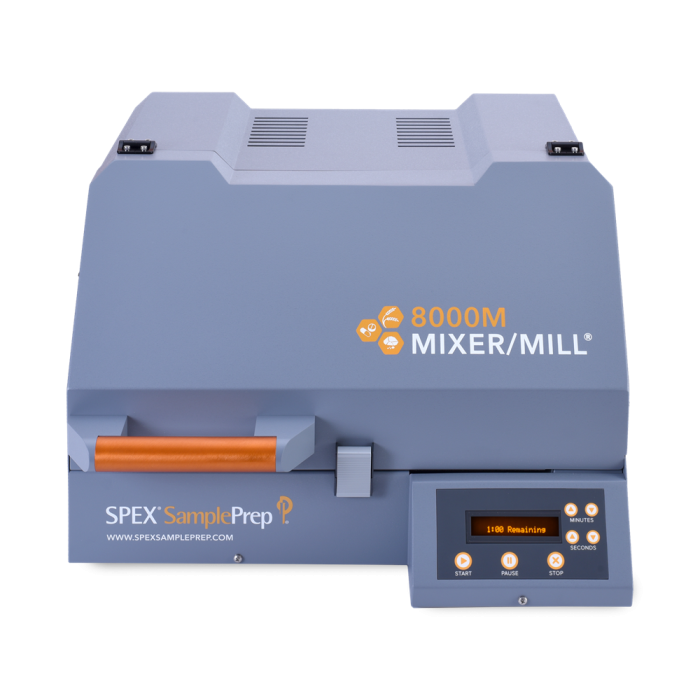
\includegraphics[height=0.8\pageheight]{figuras/big.png} \note<1>{Este es un molino de bolas SPEX}
            \onslide<2> 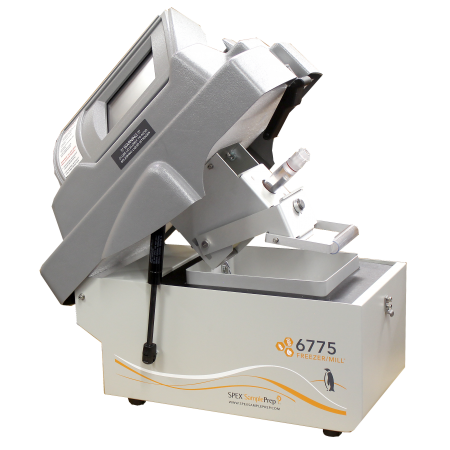
\includegraphics[height=0.8\pageheight]{figuras/cryo.png}
            \note<2>{Este es un molino SPEX con capacidad de mantener temperaturas criogénicas.}
        \end{overprint}
        \end{center}
    \end{figure}
    \end{columns}
\end{frame}

\begin{frame}{Comparación de capacidades}
\begin{longtblr}[%
    caption = {\small Comparación de tipos de molinos convencionales en función a cantidades de material que pueden procesar.},
    % entry = {Short Caption},
    label = {tbl:TipoDeMolino}]
    {%
    colspec = {XX}, width = 0.85\linewidth,
    rowhead = 1
    }
    \toprule
    Tipo de molino & Tamaño de muestra \\ \midrule
    Molino mezclador & Hasta dos de \qty{20}{\gram} \\
    Molino planetario & Hasta cuatro de \qty{250}{\gram} \\
    Molino de atrición & \qtyrange{0.5}{100}{\kilo\gram} \\
    Molino de bolas & Hasta cuatro de \qty{2000}{\gram} \\ \bottomrule
\end{longtblr}
\end{frame}

\subsection{Contenedor del molino}

\begin{frame}{Importa el material del contenedor}
\begin{itemize}
    \item \emph{El material} del contenedor del molino es un factor muy importante a considerar.
    \begin{enumerate}
        \item<2-> Puede influir en \emph{que tan contaminada} pueda estar nuestra fase metaestable.
        \item<3-> Si ambos tienen el mismo material, puede alterar la composición química del polvo.
    \end{enumerate}
\end{itemize}
\end{frame}

\begin{frame}{Materiales convencionales}
    Entre los materiales más comunes para contenedores con aplicaciones en molinos se encuentran:
    \begin{itemize}[<+-| alert@+>]
        \item acero reforzado;
        \item acero cromado reforzado;
        \item acero templado;
        \item acero inoxidable;
        \item \ch{WC-Co}
        \item acero recubierto de \ch{WC}.
    \end{itemize}
\end{frame}

\begin{frame}{Materiales para propósitos especiales}
    \begin{columns}\note{Se pueden usar contenedores de materiales especializados}
        \column{0.38\linewidth}
        \small
    Contenedores de materiales para propósitos especializados:
    \begin{itemize}
        \item<1-> cobre;
        \item<2-> titanio;
        \item<3-> safíro;
        \item<4-> agata;
        \item<5-> porcelana dura;
        \item<6-> \ch{Si3N4}
        \item<7-> \ch{Cu-Be}
    \end{itemize}
    \column[c]{0.58\linewidth}
    \begin{figure}
        \begin{center}
        \begin{overprint}
            \onslide <1>\pgfimage[width=\linewidth]{./figuras/materiales/cu.jpg}
            \onslide <2>\pgfimage[width=\linewidth]{./figuras/materiales/ti.jpg}
            \onslide<3>\pgfimage[width=\linewidth]{./figuras/materiales/zap.jpg}
            \onslide<4>\pgfimage[width=\linewidth]{./figuras/materiales/aga.jpeg}
            \onslide<5>\pgfimage[width=\linewidth]{./figuras/materiales/por.jpg}
            \onslide<6>\pgfimage[width=\linewidth]{./figuras/materiales/sin.png}
            \onslide<7>\pgfimage[width=\linewidth]{./figuras/materiales/cube.jpg}
        \end{overprint}
        \end{center}
    \end{figure}
    \end{columns}
\end{frame}

\subsection{Forma del contenedor}

\begin{frame}{Forma del contenedor}
\begin{itemize}
    \item<1-> La forma del contenedor puede afectar en los tiempos de molienda drasticamente.
    \item<2-> para los molinos SPEX existen \emph{contenedores de fondo plano} y \emph{contenedores de fondo redondo}
    \item<3-> El tiempo requerido para que se llegara a la misma intensidad en un pico en XRD en (111) fue de:
    \begin{enumerate}
        \item \qty{9}{\hour} en el contenedor de fondo plano;
        \item \qty{15}{\hour} en el contenedor de fondo redondo.
    \end{enumerate}
\end{itemize}
\end{frame}

\begin{frame}{Forma del contendor}

    \begin{figure}
        \centering
        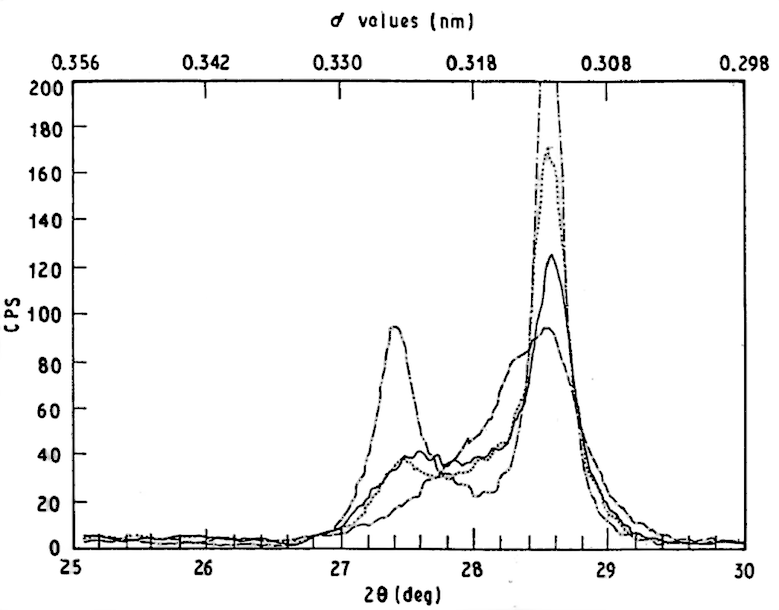
\includegraphics[height=0.7\pageheight,keepaspectratio]{figuras/efectoXRD-ed.png}
        \caption{\footnotesize Efecto del uso de un contenedor de fondo plano vs uno de fondo redondo. (-.-) \qty{3}{\hour} y (\(\cdots\)) \qty{6}{\hour} en vial redondo; (---) \qty{3}{\hour} (-\ -\ -) \qty{6}{\hour} en vial con fondo plano. \textit{(Obtenido de \cite{harringaEffectsVialShape1992}).}}
    \end{figure}
\end{frame}

\subsection{Velocidad/intensidad de molienda}

\begin{frame}{Velocidad de molienda}
    \begin{tcolorbox}[title={Velocidad crítica, \(C_s\):}]
        \small
        En un molino de bolas, la \emph{velocidad crítica (\(C_s\))} es la velocidad en la que el medio de molienda se adhiere, a causa de la fuerza centrífuga, a las paredes del contenedor.
        
        La fórmula de la velocidad crítica es:

        \begin{equation}
            C_s = \frac{\pi}{2}\sqrt{\frac{g}{R-r}}
        \end{equation}

        Donde \(g\) es la constante gravitacional, \(R\) es el diámetro interno del molino y \(r\) el diámetro de un trozo de medio de molienda. 
    \end{tcolorbox}
\end{frame}

\begin{frame}{Velocidad crítica del molino}
    \begin{itemize}
        \item<1-> A velocidades mayores que la \textit{velocidad crítica} las bolas estarían sujetas al contenedor y no causarían ningún impacto;
        \item<2-> la velocidad debe ser ajustada para que sea menor que la \emph{velocidad crítica.} 
    \end{itemize}

    \begin{figure}
        \centering
        \includegraphics<1->[width=0.9\linewidth]{figuras/Cs/vel1.jpeg}
    \end{figure}
\end{frame}

\begin{frame}{Rangos de operación}
    \begin{itemize}[<+-| alert@+>]
        \item Los molinos de bolas secos operan en un rango de \qtyrange{50}{70}{\percent} de la \(C_s\);
        \item normalmente se operan de \qtyrange{60}{65}{\percent};
        \begin{enumerate}
            \item a \qty{\le 50}{\percent} \(C_s\) la enrgía es muy poca para \emph{fracturar el polvo;}
            \item a \qty{\geq 70}{\percent} \(C_s\) el medio comienza a caer en \emph{catarata,} golpeando una sola zona del contenedor.
        \end{enumerate}
    \end{itemize} 
\end{frame}

\begin{frame}{Temperatura del medio}
    Una de las consecuencias de moler a \emph{altas velocidades} es que la \emph{temperatura del medio aumenta.}
\end{frame}

\begin{frame}{Ventajas de una mayor velocidad}
    \begin{itemize}
        \item Puede promover la homogeneidad y/o aleaciones de polvos.
    \end{itemize}
\end{frame}

\begin{frame}{Desventajas de una mayor velocidad}
    \begin{itemize}[<+-| alert@+>]
        \item acelera la transformación del proceso, resultando en descomposición de la fase deseada;
        \item se pueden formar otras fases metaestables indeseadas;
        \item incrementa el riesgo de contaminación de polvos.
    \end{itemize}
\end{frame}

\begin{frame}{Obtención de fases en función de la velocidad}
    En algunas investigaciones, se han reportado \emph{cambios en la morfología} en función de la \emph{velocidad}:\footcite{calkaUniversalHighPerformance1991}\note{En algunas investigaciones se ha reportado que a diferentes velocidades se producen diferentes fases}
    \medskip
    \begin{longtblr}[caption={Relación de la velocidad con las fases obtenidas}]{colspec = {XX}, width = 0.85\linewidth, rowhead = 1}
    \toprule 
    Fase obtenida & Velocidad de molienda \\ \midrule
    \ch{Ni-Zr} (amorfo) & Alta velocidad \\
    \ch{Ni-Zr} (cristalino) & Velocidad media y baja \\
    \bottomrule    
    \end{longtblr}
\end{frame}

\subsection{Tiempo de molienda}

\begin{frame}{Factores que influyen en el tiempo de molienda}

\begin{itemize}
        \item Es el factor más importante;
        \item el tiempo de molienda depende de:
            \begin{enumerate}
                \item tipo de molino;
                \item intensidad de molienda;
                \item \gls{BPR};
                \item temperatura de molienda.
            \end{enumerate}
    \end{itemize}
\end{frame}

\begin{frame}{Desventajas de un mayor tiempo de molienda}
    \begin{itemize}
        \item<1-> Se debe de limitar el tiempo de \emph{molienda solo al necesario}\footcite{suryanarayanaDoesDisorderedGTiAl1995}
        \item<2-> \alert<2>{A mayor tiempo de molienda, más posibilidad de contaminación.}
        \item<3-> \alert<3>{Mayor posibilidad de degradar el polvo.}
    \end{itemize}
\end{frame}

\begin{frame}{Precauciones adicionales}
    \begin{itemize}
        \item Hay mayor contaminación a mayor tiempo de molienda;
        \item esto es especialmente aplicable a contenedores/medios de molienda reactivos, como:\footcite[64]{suryanarayanaMechanicalAlloyingMilling2004}
        \begin{itemize}
            \item \ch{Ti};
            \item \ch{ZrO2}.
        \end{itemize}
    \end{itemize}
\end{frame}

\subsection{Medio de molienda}

\begin{frame}{Selección del medio de molienda}
    \begin{itemize}
        \item Una correcta selección del medio de molienda es crucial;\note{también hay que considerar para el medio}
        \begin{itemize}
            \item tamaño;
            \item distribución de tamaños.
        \end{itemize}
    \end{itemize}
\end{frame}

\begin{frame}{Medios de molienda convencionales}
    Entre los materiales más comunes para su uso en medios de molienda, se encuentran:
    \begin{itemize}
        \item acero reforzado;
        \item acero;
        \item acero cromado reforzado;
        \item acero templado;
        \item acero inoxidable;
        \item \ch{WC-Co};
        \item acero para rodamientos. 
    \end{itemize}\note{La selección del medio de molienda generalmente se hace conforme a la densidad, ya que un material más denso, proporcionaría una mayor fuerza de impacto al polvo.}
\end{frame}

\begin{frame}{Medios de molienda especializados}
    Así como con los contenedores, también se pueden usar medios de molienda para usos especializados:
    \begin{itemize}[<+-| alert@+>]
        \item cobre;
        \item titano;
        \item niobio;
        \item zirconia (\ch{ZrO2})
        \item ágata;
        \item \gls{YSZ};
        \item zafiro;
        \item nitruro de silicio (\ch{Si3N4});
        \item \ch{Cu-Be};
    \end{itemize}
\end{frame}

\begin{frame}
    \begin{itemize}
        \item<1-> Se ha determinado que en \alert<2>{condiciones suaves} de molienda (bolas más pequeñas, menor energía y menor \gls{BPR}) favorece la formación de \alert<2>{fases metaestables.\footcite{suryanarayanaPhaseSelectionMechanically1999}}
        \item<2-> por el contrario, al usar \alert<3>{condiciones más duras,} se favorece la formación de \alert<3>{fases menos metaestables o de fases en equilibrio.\footcite{gerasimovTribochemicalEquilibriumMechanical1991}}
    \end{itemize}
\end{frame}

\subsection{Relación de bolas-polvo (BPR)}

\begin{frame}{BPR en función del tamaño de muestra}
    \begin{itemize}
        \item Se ha estudiado de 1:1\footcite{chinAmorphizationNiSiCTernary1996} hasta 220:1\footcite{kis-vargaPhaseTransitionsCuSb1996}
        \item normalmente se usa una \gls{BPR} de 10:1 para molimos de poca capacidad como un SPEX;
        \item para attritores se puede usar desde 50:1 hasta 100:1
    \end{itemize}
\end{frame}

\begin{frame}{BPR en función del tiempo}
    \begin{itemize}
        \item A \alert<1->{mayor BPR,} \alert<1->{menor tiempo} de molienda
    \end{itemize}

    \begin{longtblr}[caption={Variación de BPR y el tiempo necesario para sintetizar Ti-33\%Al amorfo.},label={tbl2}]{%
        colspec = {XX},
        rowhead = 1
        }
        \toprule
        BPR & Tiempo \\ \midrule
        10:1 & \qty{7}{\hour} \\
        50:1 & \qty{2}{\hour} \\ \bottomrule
    \end{longtblr}
\end{frame}

\begin{frame}{Condiciones de molienda y su influencia en las fases obtenidas}
    \begin{tcolorbox}[title={Condiciones de molienda}]
        \bigskip
        \begin{longtblr}[caption={Condicones de molienda y fases obtenidas.}]{width=0.8\linewidth, colspec={X[1,c]X[1.5,c]}, rowhead=1}
        \toprule
        \textbf{Condiciones de molienda} & \textbf{Fase obtenida} \\ \midrule
        \emph{Suaves} & fases metaestables \\ \note{condiciones suaves son un bajo BPR, baja velocidad, etc.}
        \emph{Duras} & fases en equilibrio \\ \bottomrule
        \end{longtblr}
    \end{tcolorbox}
\end{frame}

\begin{frame}
    \begin{figure}
        \centering
        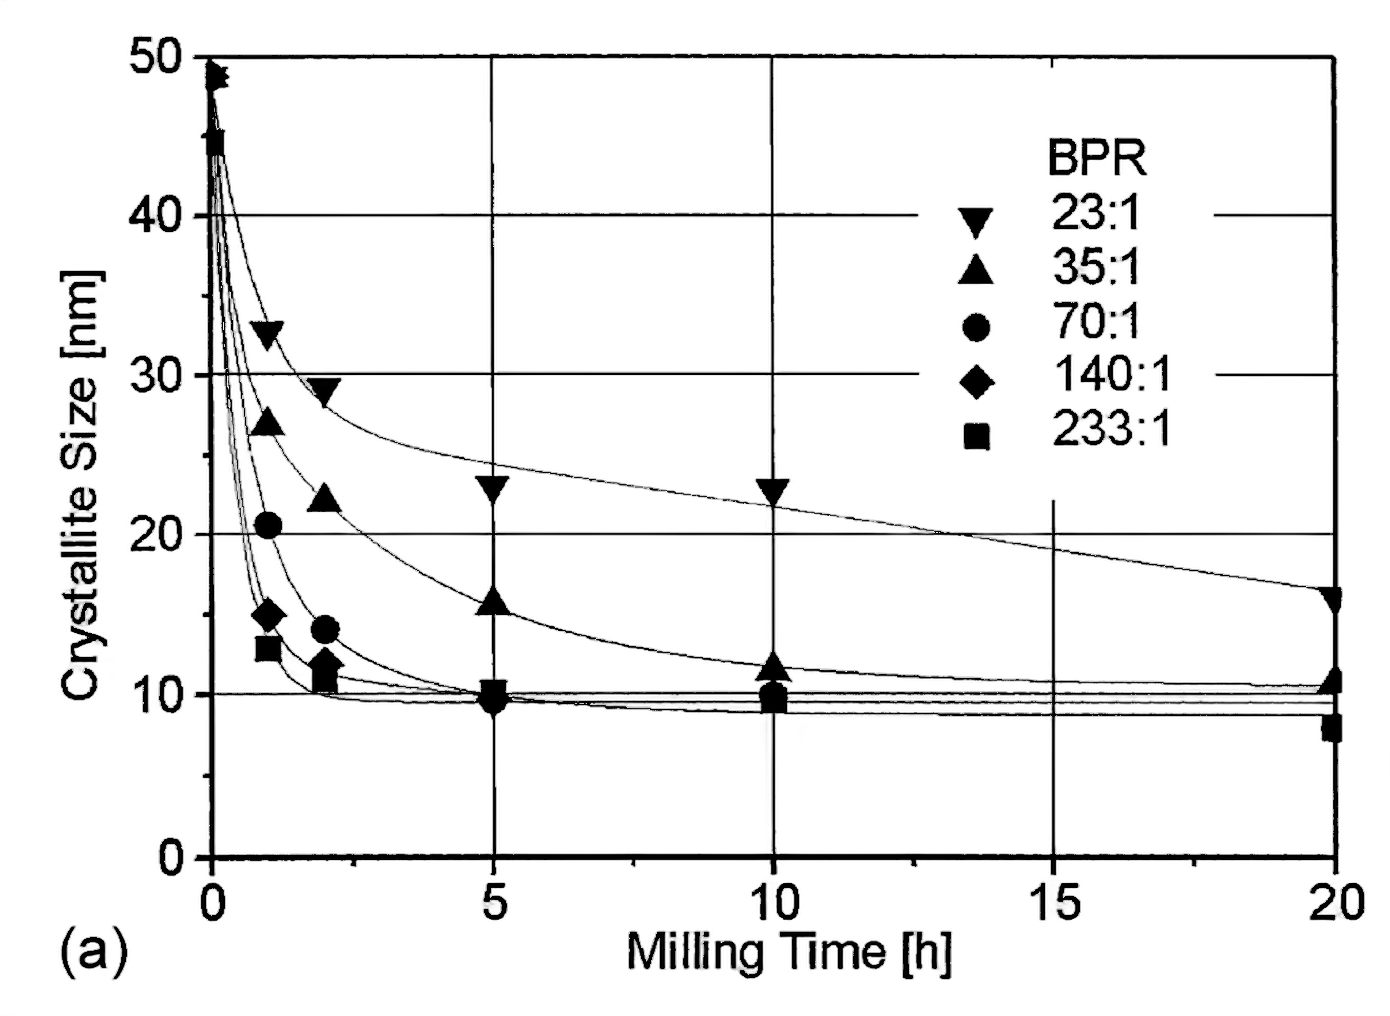
\includegraphics[height=0.8\pageheight]{figuras/suryanarayana2004p68-a.png}
        \caption{Influencia del BPR en el tamaño del polvo a diferentes tiempos. \textit{(Adaptado de \textcite[68]{suryanarayanaMechanicalAlloyingMilling2004}).}}
    \end{figure}
\end{frame}

\begin{frame}
    \begin{figure}
        \centering
        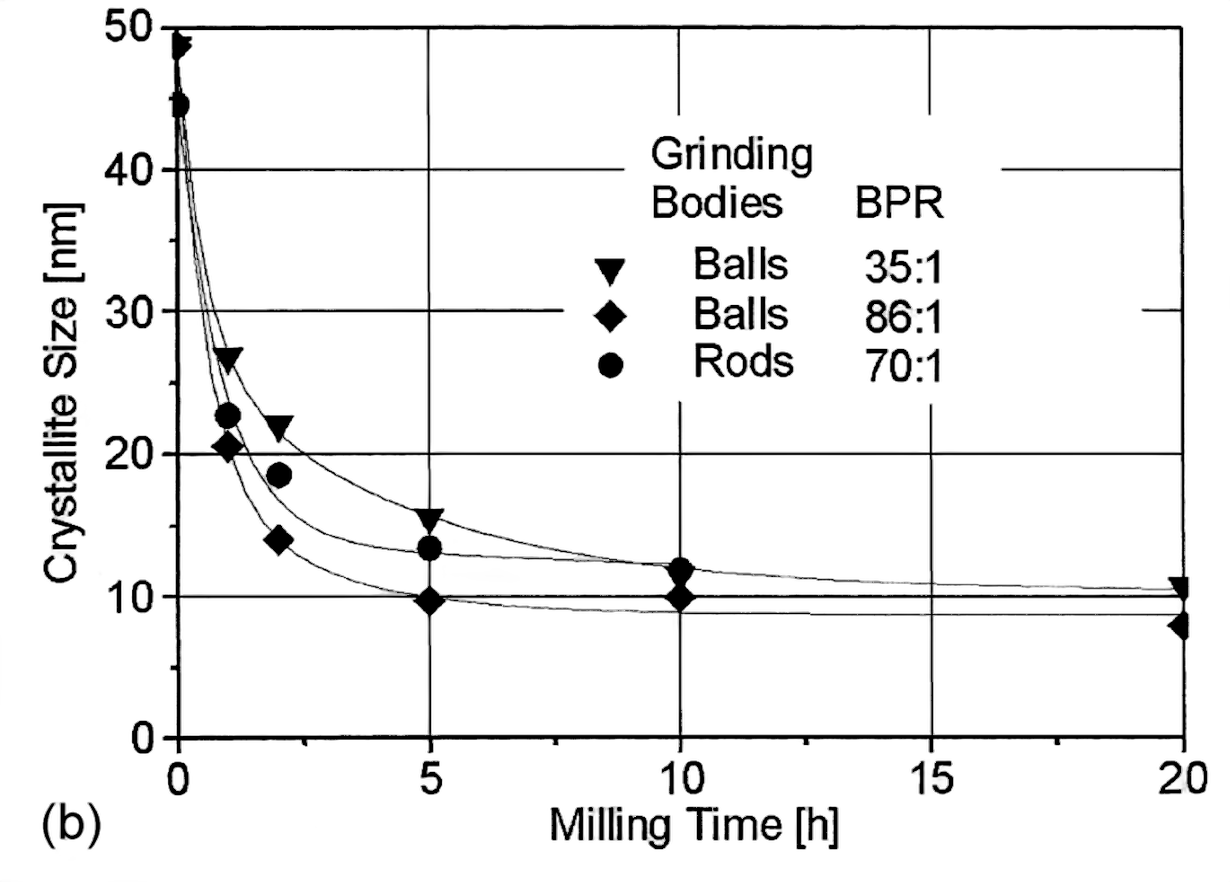
\includegraphics[height=0.8\pageheight]{figuras/suryanarayana2004p68-b.png}
        \caption{Influencia del BPR  y la forma del medio de molienda en el tamaño del polvo a diferentes tiempos. \textit{(Adaptado de \textcite[68]{suryanarayanaMechanicalAlloyingMilling2004}).}}
    \end{figure}
\end{frame}

\subsection{Grado de llenado del vial}

\begin{frame}{Consideraciones generales}
    \begin{itemize}
        \item Ya que la molienda depende del impacto de las bolas con el polvo, no puede llenarse por completo el vial;
        \item se recomienda llenarlo \qty{\leq 50}{\percent}.
    \end{itemize}
\end{frame}

\subsection{Atmósfera de molienda}

\begin{frame}{La influencia de la atmosfera de molienda}
    \begin{itemize}
        \item Es de los principales contribuyentes a la contaminación;
        \item se evita llenando con gas inerte el contenedor;\note{Se prefiere el uso de argón o helio.}
        \item comúnmente se usa argón para evitar la oxidación.
    \end{itemize}
\end{frame}

\begin{frame}{Uso de otros gases}
    \begin{itemize}
        \item \emph{No es común} que se use nitrógeno;
            \begin{enumerate}
                \item \emph{se puede utilizar} nitrógeno o amoníaco para \emph{producir nitruros;\footcite{calkaSynthesisNitridesMechanical1992}}
                \item \emph{se puede uitlizar} hidrógeno para \emph{producir hidruros.\footcite{chenHydridingReactionsInduced1996}}
            \end{enumerate} 
    \end{itemize}
\end{frame}

\begin{frame}{Morfología de la fase obtenida}
    \begin{itemize}
        \item La atmósfera puede influir en la morfología obtenida:
        \item \textcite{oginoNonequilibriumPhasesFormed1990} determinó que para la preparación de \ch{Cr-Fe}: 
        \begin{enumerate}
            \item en atmósfera de argón se presentaban picos de XRD correspondientes a \ch{Cr};
            \item en aire-Ar y en nitrógeno se formaba una fase amorfa.
        \end{enumerate}
    \end{itemize}
\end{frame}

\begin{frame}
    \begin{figure}
        \centering
        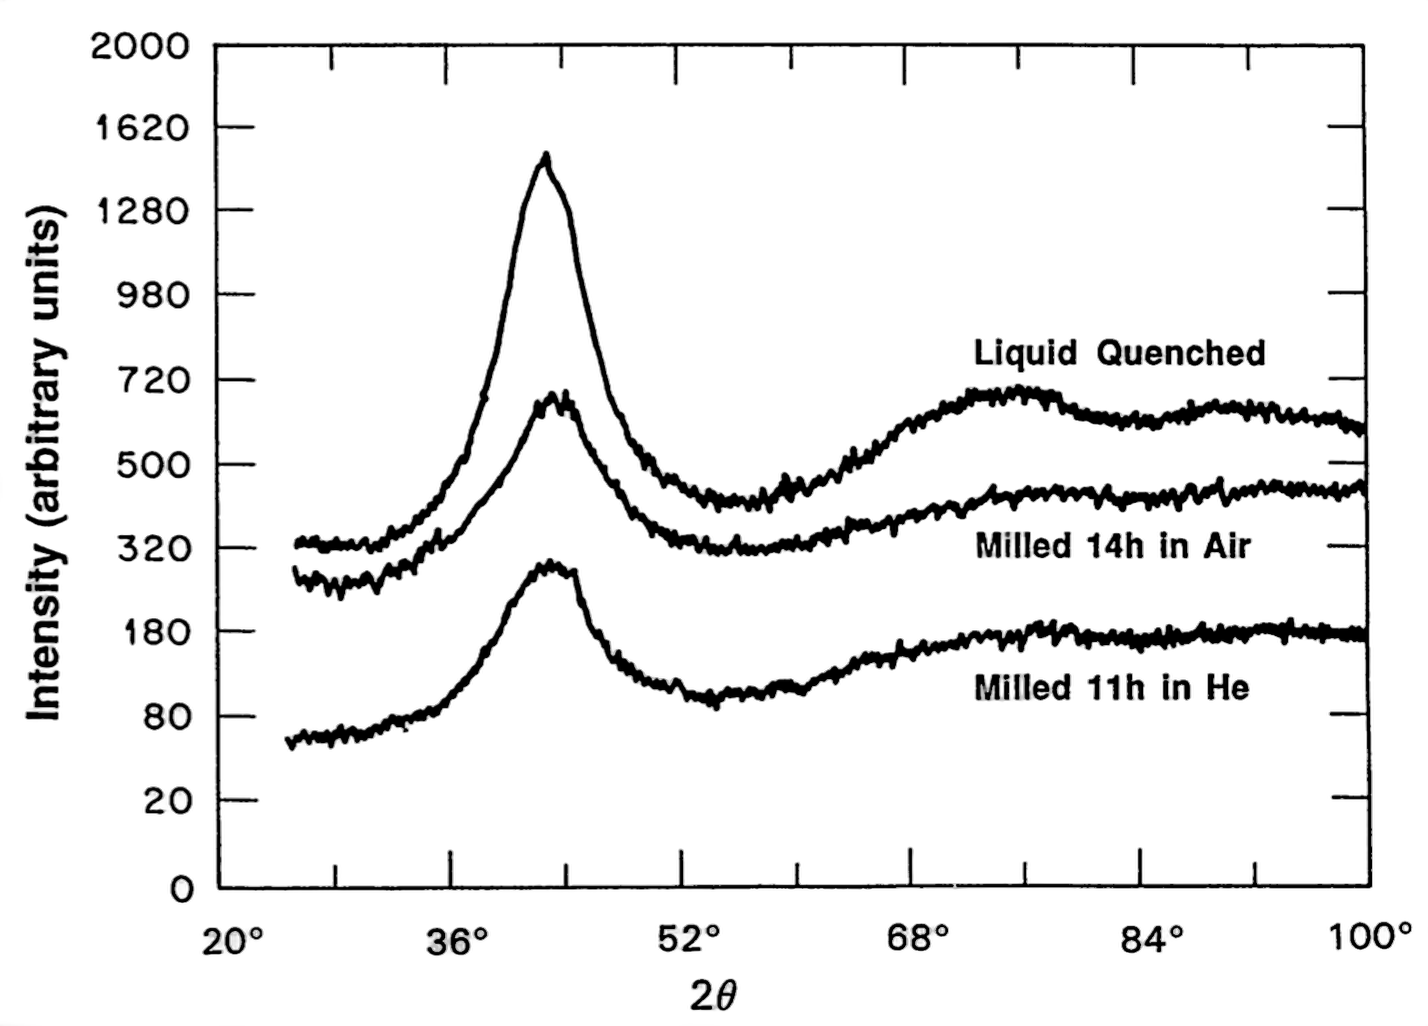
\includegraphics[height=0.8\pageheight]{figuras/Koch1995-XRD-a.png}
        \caption{Efecto de la atmosfera en la cristalinidad del polvo.}
    \end{figure}
\end{frame}

\subsection{Agentes de control del proceso (PCA)}

\begin{frame}{Prevención de soldadura en frío}
    \begin{itemize}
        \item Solo se puede obtener una aleación adecuada si se mantiene una relación adecuada entre fracturas de partículas y soldadura en frío;
    \end{itemize}
\end{frame}

\begin{frame}{Uso de PCA}
\begin{itemize}
    \item Se usan \gls{PCA} para reducir la soldadura en frío;
    \begin{itemize}
        \item estos pueden ser sólidos, líquidos o gases;
        \item el \gls{PCA} se absorbe en la superficie del polvo
        \item inhibe la aglomeración
    \end{itemize} 
    \item en práctica, se usa \qtyrange{1}{5}{\percent}m.
\end{itemize}
\end{frame}

\subsection{Temperatura}

\begin{frame}{La temperatura define la constitución}
    \begin{itemize}
        \item<1-> La difusión es un proceso involucrado en la formación de las fases;
        \begin{itemize}
            \item<2-> a mayor temperaturas:\footcite{hongSteadyStateGrain1994}
            \begin{itemize}
                \item<3-> se obtienen menor RMS del estrés de las nanopartículas;
                \item<4-> menor tamaño de grano.
            \end{itemize} 
            \item<5-> a menor temperatura:\footcite{kimuraProcessingControlSolid1989}
            \begin{itemize}
                \item<6-> hay evidencia contradictoria, pero en teoría se favorece la \emph{amorficidad.}
            \end{itemize}
        \end{itemize}
    \end{itemize}
\end{frame}

\begin{frame}[allowframebreaks]{Referencias}
    \small
    \printbibliography
\end{frame}

\end{document}